\section{Background}
\label{sect.background}

Distributed systems are conventionally modeled as a set of \emph{nodes} (or \emph{processes}) that
can communicate only by sending and receiving messages over a network. In practice, nodes may be
servers in datacenters, end-user devices such as laptops and smartphones, or any other kind of
device with network connectivity. We assume that messages sent via the network may be delayed,
reordered, or lost entirely~-- an assumption that matches the behavior of many networks in practice
\cite{Bailis:2014jx}.

Moreover, nodes or network links may fail at any time, and the non-faulty parts of the system need
to continue working in spite of such partial failures. Programming such systems is far more
difficult than writing programs that execute on a single machine. Consequently, it is valuable for
application developers to have access to abstractions that simplify the development of distributed
programs. The \emph{collaborative editing} (or \emph{data synchronization}) model discussed in this
paper is an example of such an abstraction.

The goal of an abstraction for distributed programming is to provide certain guarantees that hold in
all possible executions of a system, so that higher-level programs may rely on the abstraction
without having to worry about how it is implemented. In this paper, the abstraction we discuss is
\emph{replicated data}, that is, ensuring that each replica node has a local copy of some data
structure (such as a document). Each node may independently read and modify the data, and any
updates (modifications) are propagated to other replicas via the network.

\subsection{Consistency Models for Replicated Data}\label{sect.consistencymodels}

The purpose of replication is to ensure that you have a copy of the same data on each node that is
acting as a replica. However, when multiple nodes are concurrently reading and modifying the data,
they do not have a single shared view of the data, since each node only has direct access to its
local storage, and can observe the state of another node only by exchanging messages with it via the
unreliable network \cite{Sheehy:2015jm}.

For this reason, it is likely that at any given moment in time, two replicas are not in the same
state, for example because one has received a message that has not yet been delivered to the other.
A replication algorithm must ensure that nevertheless, all replicas eventually end up in the same
state. In order to describe how and when this happens, a \emph{consistency model} defines the
guarantees provided by the replication algorithm.

\subsubsection{Strong and Eventual Consistency}

There is a spectrum of consistency models that are used in practice
\cite{Terry:1994fp}, with the two extremes of the spectrum being \emph{strong} and \emph{eventual}
consistency, respectively:

\begin{description}
\item[Strong consistency] in the context of replicated data is usually understood as linearizability
\cite{Herlihy:1990jq,Gilbert:2002il}. A linearizable system can be informally described as follows:
each operation takes effect atomically at one moment in time, and concurrent operations behave as if
there were only one copy of the data, even if in reality each replica has a separate copy. In
particular, after a write has completed, all subsequent reads must return the written value (or a
later one), since that is the behavior of a single memory location without caching or buffering. In
the context of databases, strong consistency typically refers to serializable isolation and
transaction atomicity \cite{Davidson:1985hv}.
\item[Eventual consistency] is less formally defined than linearizability, but is usually described
as ``if no new updates are made to an object, eventually all reads will return the last updated
value'' \cite{Bailis:2013jc,Burckhardt:2014hy,Terry:1994fp,Vogels:2009ca}. However, this property is
very weak: it does not define what happens if the updates to the object never cease, nor does it
constrain the values that reads may return before consistency is eventually reached.
\end{description}

The spectrum of consistency models exists due to a trade-off: systems with stronger guarantees may
have lower performance or be less fault-tolerant than systems with weaker guarantees
\cite{Davidson:1985hv,Terry:1994fp,Gilbert:2002il}. However, it is possible to strengthen the
guarantees of eventual consistency without incurring the costs inherent in strong consistency.

\subsubsection{Strong Eventual Consistency (SEC)}

One such intermediate consistency model for replicated data is \emph{strong eventual consistency} or
SEC \cite{Shapiro:2011un}. It has performance and fault-tolerance characteristics that are similar
to eventual consistency, but provides stronger guarantees. An algorithm providing SEC is defined as
satisfying the following properties:

\begin{description}
\item[Convergence:] Correct replicas that have delivered the same updates have equivalent state.
\item[Eventual delivery:] An update delivered at some replica is eventually delivered to all correct
replicas.
\item[Termination:] All executions of the algorithm eventually terminate.
\end{description}

A node is defined to be \emph{correct} if it is not faulty, i.e. if it does not crash and if it is
not permanently disconnected from the network. Although the network may be interrupted for periods
of time, a correct node will eventually be able to communicate with other correct nodes, and so the
eventual delivery property can be achieved by re-sending messages until they arrive. A faulty node
is by definition not required to deliver any messages. Termination is also straightforward to show
for many algorithms.

Thus, the key correctness property for SEC is \emph{convergence}. It is a safety property
\cite{Alpern:1985dg}~-- that is, it must hold at every point in the execution: whenever two replicas
have seen the same set of updates, but perhaps in a different order, they must be in an equivalent
state. Two states are equivalent if all reads return the same result in both states. Convergence is
much stronger than eventual consistency (a liveness property), since the definition of convergence
constrains the values that reads may return at any time, even if the system is never quiescent.

\subsection{Properties of Networks}\label{sect.background.networks}

The consistency properties that a replication algorithm can achieve depend on the assumptions that
can be made about the network and its connectedness.

\subsubsection{Asynchronous System Model}

In this paper, we discuss an approach for achieving SEC in \emph{asynchronous} systems. In the
asynchronous system model, we make no timing assumptions at all: messages may suffer unbounded
network delays, and nodes may stop executing for unbounded periods of time or fail completely
\cite{Cachin:2011wt}. Our formal definition of the asynchronous model appears in
Section~\ref{sect.network}.

Although most practical systems have fairly low network delay and fairly brief execution pauses most
of the time \cite{Bailis:2014jx}, the asynchronous model is a useful lower bound for the assumptions
that a distributed algorithm may make. Any algorithm that is proved correct under the assumptions of
the asynchronous model is also guaranteed to be correct in a system that provides stronger
guarantees, for example around timing and reliability.

Some guarantees cannot be provided in the asynchronous model; for example, there is no consensus
algorithm that is guaranteed to terminate in this system model \cite{Fischer:1985tt}. On the other
hand, consensus becomes possible if the algorithm is allowed to make certain weak timing assumptions
\cite{Chandra:1996cp}. However, SEC \emph{can} be achieved in the asynchronous model, so we use it
here in order to keep our assumptions minimal.

\subsubsection{Centralized Versus Peer-to-Peer Networks}

Many online services today rely on a central server that maintains the authoritative copy of the
data. In this architecture, clients that want to modify the data send their updates to the central
server (often called \emph{master} or \emph{leader}), which in turn forwards the updates to all of
the replicas. The server can attach a sequence number to each update, enabling all replicas to apply
the updates in the same order. Being able to assume totally ordered delivery across all replicas
significantly simplifies replication algorithms, which is why this architecture is so popular today.

As discussed in Section~\ref{sect.introduction}, peer-to-peer networks have no such central server
that can be assumed to be always reachable. It is possible to provide the same ordering guarantee in
peer-to-peer networks; this abstraction is known as \emph{total order broadcast} or \emph{atomic
broadcast} \cite{Cachin:2011wt}. However, it is expensive: total order broadcast is equivalent to
consensus \cite{Chandra:1996cp}, making it unattainable in the asynchronous model. Even if we
introduce timing assumptions, total order broadcast requires a quorum of nodes (typically a
majority) to be reachable in order to make progress; in a peer-to-peer network of mobile devices, it
is likely that less than a majority of devices is online at any one time, and so an algorithm for
total order broadcast would be stalled.

If we require any subset of nodes to be able to synchronize data independently from the remaining
nodes (for example, two devices connected by a wireless link but disconnected from the internet), we
cannot rely on total order broadcast. In this setting, causally ordered delivery is the strongest
guarantee that can reliably be provided \cite{Attiya:2015dm}.

\subsubsection{Causal Ordering}

Total order broadcast ensures that when nodes broadcast a set of messages to other nodes on the
network, they are delivered in the same order to all recipients. By contrast, causal ordering is a
weaker guarantee that allows greater concurrency and thus greater nondeterminism in the network.
However, it has the advantage that it makes no assumptions about the number of nodes that are
online.


% There are two families of algorithms for collaborative editing: \emph{operational transformation}
% (OT)~\cite{Ellis:1989ue,Ressel:1996wx,Oster:2006tr,Sun:1998vf,Sun:1998un,Suleiman:1998eu,Nichols:1995fd}
% and \emph{conflict-free replicated datatypes}
% (CRDTs)~\cite{Shapiro:2011wy,Roh:2011dw,Preguica:2009fz,Oster:2006wj,Weiss:2010hx,Nedelec:2013ky,Kleppmann:2016ve}.
% Both allow a document to be modified concurrently on different replicas, with changes applied
% immediately to the local copy, while asynchronously propagating changes to other replicas. The
% goal of these algorithms is to ensure that for all concurrent executions, the replicas converge
% toward the same state without any edits being lost, a property known as \emph{strong eventual
% consistency}~\cite{Shapiro:2011un}.


% CRDTs are a more recent development~\cite{Shapiro:2011un}. While OT is based on transforming
% non-commutative operations so that they have the same effect when reordered, CRDTs define operations
% in a way that makes them commutative by design, making them more amenable to peer-to-peer settings
% in which each node may apply edits in a different order. CRDTs also have attractive performance
% characteristics~\cite{Mehdi:2011ke}.

% TODO Various decentralised algorithms have been proposed and all but one (Oster 2006) have
% subsequently been shown to be incorrect.


\subsection{Collaborative Editing and Data Synchronization}\label{sect.datasync}

In a strongly consistent system, as long as a node is disconnected (also known as
\emph{partitioned}) from all other nodes, read and write operations cannot return on that node,
because they need to wait for communication with other nodes to complete in order to find out about
writes that occurred on other nodes. This observation is popularly known as the CAP theorem
\cite{Gilbert:2002il}, and it makes linearizability impossible for applications that need to
continue working if a network connection is slow or unavailable.

On the other hand, SEC systems can serve reads and writes entirely from a local replica without
waiting for network communication, and exchange updates with other replicas asynchronously when a
network connection is available. For example, this mode of data exchange is familiar from calendar
sync on mobile devices: a user can view and enter calendar entries while the device is offline, and
any changes are propagated to replicas of the calendar on other devices when an internet connection
is available.

\subsubsection{The Need for Conflict Resolution}

In SEC systems, different replicas may concurrently execute conflicting operations without being
aware of each other, causing their states to diverge, and requiring \emph{conflict resolution}
(reconciliation) at a later time. Some systems place the burden of conflict resolution on the user,
or leave it to application code, which is often error-prone (for example, \citet{DeCandia:2007ui}
describe an anomaly at Amazon that arose due to poor conflict resolution). The definition of SEC
requires convergence, which implies automatic conflict resolution: the replication algorithm must
ensure that once the updates have been propagated, the states of replicas are equivalent.

The simplest way of achieving convergence is a \emph{last write wins} (LWW) policy, in which a
unique timestamp is assigned to each version of the data structure, and when there is a conflict,
the system picks the version with the highest timestamp. In this approach, concurrent updates with a
lower timestamp are simply discarded. Better algorithms are able to preserve concurrent updates
while still ensuring automatic convergence.

\subsubsection{Conflict-Free Replicated Data Types (CRDTs)}

Some operations, such as addition of numbers, are naturally commutative. Thus, if the replicated
data structure is a counter whose value can only be incremented or decremented, convergence can be
achieved by applying the increment and decrement operations in any order at each replica.

\emph{Conflict-free replicated data types} (CRDTs) generalize this idea to other data structures and
operations
\cite{Shapiro:2011wy,Shapiro:2011un,Roh:2011dw,Preguica:2009fz,Oster:2006wj,Weiss:2010hx,Nedelec:2013ky,Kleppmann:2016ve}.
For example, an ordered list (sequence) of values can be modified by inserting or deleting elements
at specified positions, and a map (dictionary) datatype can be modified by setting the value
associated with a key or deleting a key-value pair from the map. In a CRDT, those modification
operations are made commutative by attaching additional metadata to the data structure.

Three families of CRDTs are distinguished in the literature:
\begin{description}
\item[Operation-based CRDTs] construct update operations such that they are commutative. Every
update operation that is performed on one replica is broadcast to other replicas, where the
operation is applied when it is delivered. Due to the commutativity of operations, replicas converge
towards the same state, even when each node applies the operation in a different order.
\item[State-based CRDTs] do not capture individual update operations, but instead broadcast the
entire state of a replica after it has changed. The CRDT defines a \emph{merge} function over a
join-semilattice, allowing states to be combined such that the result reflects changes made in
either replica.
\item[$\delta$-CRDTs] \cite{Almeida:2015fc} are a middle ground between operation-based and state-based
CRDTs: rather than broadcasting the entire state after an update, they only send deltas reflecting
the modification. Like state-based CRDTs, $\delta$-CRDTs are based on an associative, commutative,
and idempotent merge operation, whereas operation-based CRDTs only use operation commutativity.
\end{description}

In this paper we focus on operation-based CRDTs, and in particular the RGA algorithm for ordered
lists described in Section~\ref{sect.rga.background}. For this algorithm, we formally prove the
commutativity of operations, and prove that it achieves convergence on an asynchronous network.

\subsubsection{Operational Transformation (OT)}

Another family of algorithms for achieving convergence of replicas uses the \emph{operational
transformation} (OT) approach
\cite{Ellis:1989ue,Ressel:1996wx,Oster:2006tr,Sun:1998vf,Sun:1998un,Suleiman:1998eu,Nichols:1995fd}.
These algorithms are intended for collaborative editing, that is, multiple users concurrently
modifying a document on their local device, and propagating updates asynchronously to other users'
devices. The replicated data structure is usually assumed to be a text document, represented as an
ordered list of characters that may be modified by inserting or deleting characters at arbitrary
positions in the string.

Unlike CRDTs, in which update operations are commutative by definition, OT allows non-commutative
operations. Instead, OT relies on \emph{transforming} concurrent operations, allowing them to be
reordered on different nodes while ensuring the same outcome. For example, if two nodes started in
the same state, and then concurrently generated operations $\mathit{op}_1$ and $\mathit{op}_2$
respectively, the transformation $T$ of those operations must satisfy
\[
  T(\mathit{op}_1, \mathit{op}_2) = (\mathit{op}_1', \mathit{op}_2') \quad\text{ such that }\quad
  \mathit{op}_1 \circ \mathit{op}_2' \equiv \mathit{op}_2 \circ \mathit{op}_1' \;.
\]

This property is known as the \emph{transformation property 1} ($\mathit{TP}_1$), as defined by
\citet{Ressel:1996wx}. It allows two operations that were generated concurrently to be applied
sequentially in different orders at each replica. It is sufficient for ensuring convergence in
systems that deliver operations in the same order to all replicas, for example by sequencing them
through a central server. This design was originally pioneered by the Jupiter system
\cite{Nichols:1995fd} and is now used by all widely-deployed OT-based collaboration systems,
including Google Docs \cite{DayRichter:2010tt}, Microsoft Word Online, Etherpad
\cite{Etherpad:2011um}, and Novell Vibe \cite{Spiewak:2010vw}.

However, if the system cannot ensure that operations are delivered in the same order to all
replicas, the $\mathit{TP}_1$ property is not sufficient, and the transformation must also satisfy a
second, more subtle property $\mathit{TP}_2$ \cite{Ressel:1996wx}. This latter property has a
checkered history: several OT algorithms have claimed to satisfy $\mathit{TP}_2$, but were later
shown to be incorrect \cite{Imine:2003ks,Imine:2006kn,Oster:2005vi}. It has even been shown that in
the classic formulation of OT it is impossible to achieve $\mathit{TP}_2$ \cite{Randolph:2015gj},
and that the transformation needs to be defined differently in order to satisfy this property
\cite{Oster:2006tr}.

Hand-written proofs of the $\mathit{TP}_2$ property are laborious and difficult to check by hand
\cite{Li:2008hw,Li:2005jq}, so most algorithms have been presented without proof.
\citet{Suleiman:1998eu} developed transformation functions with a hand-written proof of
$\mathit{TP}_2$, but \citet{Oster:2005vi} showed that this proof was incorrect.
\citet{Imine:2003ks} used a theorem prover to check $\mathit{TP}_2$ for their transformation
functions, but unfortunately there was an error in the specification, as documented by
\citet{Oster:2005vi}: it relied on an assumption that was not guaranteed by the algorithm, making
the proofs invalid. Removing the incorrect assumption yielded a counterexample that violated
$\mathit{TP}_2$.

In our formalization we hope to avoid the trap of making incorrect assumptions by proving not only
the commutativity of operations, but also that the preconditions of operations are guaranteed to
hold in all executions of our network model. The network model in turn is specified by a small set
of axioms whose correctness can be robustly defended.


% We prove this convergence property in an abstract setting, that is, any two arbitrary list of
% distinct events, enriched by an order relation that satisfies a \emph{consistency property},
% converge.

\subsection{The Replicated Growable Array (RGA)}\label{sect.rga.background}

\begin{figure}
\centering
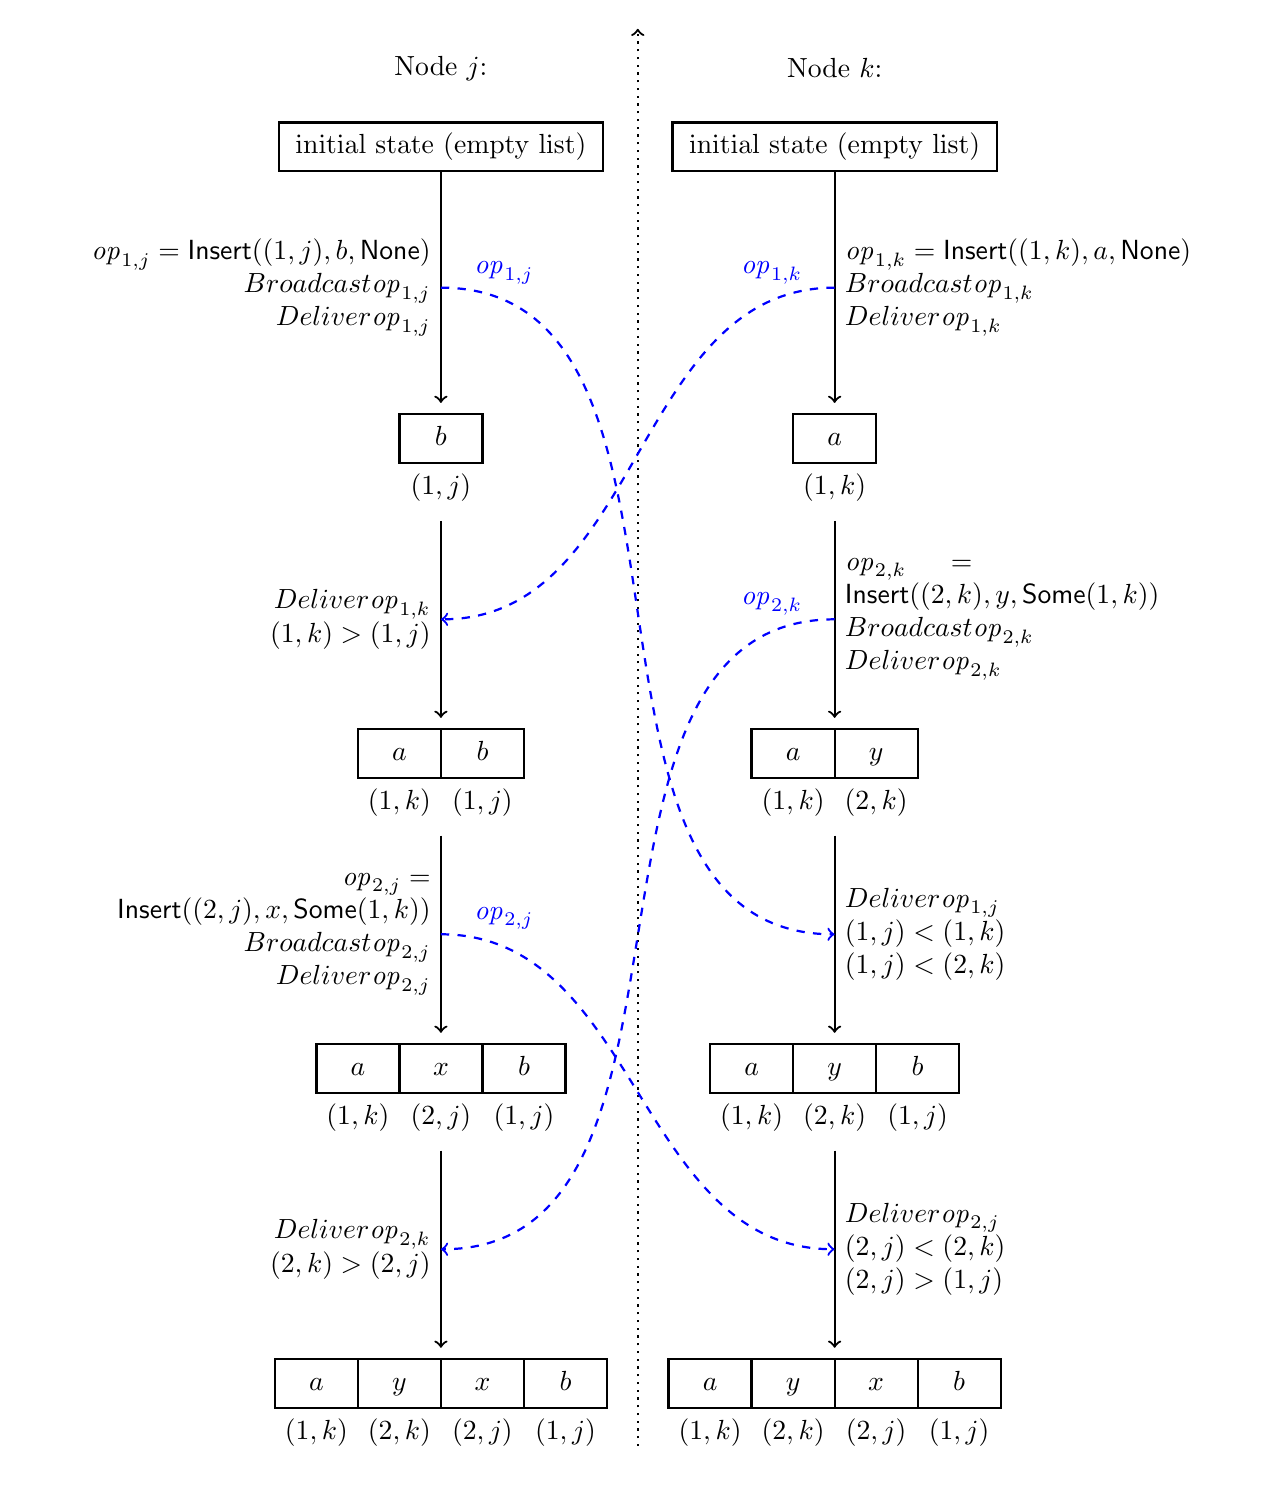
\begin{tikzpicture}[auto,scale=1.0]
\onehalfspacing
\path [draw,dotted] (2.5,-0.5) -- (2.5,17.5);

\tikzstyle{initstate}=[rectangle,draw,inner xsep=6pt,text height=8pt,text depth=3pt]
\tikzstyle{state}=[matrix,column sep={30pt,between origins}]
\tikzstyle{val}=[draw,anchor=base,minimum width=30pt,text height=8pt,text depth=3pt]
\tikzstyle{oid}=[anchor=base]
\tikzstyle{leftevent}=[left,text width=5cm,text ragged left,midway]
\tikzstyle{rightevent}=[right,text width=5cm,text ragged,midway]
\tikzstyle{every path}=[thick,->]

\node (leftR) at (0,17) {Node $j$:};
\node (left1) at (0,16) [initstate] {initial state (empty list)};
\node (left2) at (0,12) [state] {
    \node [val] {$b$};     \\
    \node [oid] {$(1,j)$}; \\
};
\node (left3) at (0,8) [state] {
    \node [val] {$a$};     & \node [val] {$b$};     \\
    \node [oid] {$(1,k)$}; & \node [oid] {$(1,j)$}; \\
};
\node (left4) at (0,4) [state] {
    \node [val] {$a$};     & \node [val] {$x$};     & \node [val] {$b$};     \\
    \node [oid] {$(1,k)$}; & \node [oid] {$(2,j)$}; & \node [oid] {$(1,j)$}; \\
};
\node (left5) at (0,0) [state] {
    \node [val] {$a$};     & \node [val] {$y$};     & \node [val] {$x$};     & \node [val] {$b$};     \\
    \node [oid] {$(1,k)$}; & \node [oid] {$(2,k)$}; & \node [oid] {$(2,j)$}; & \node [oid] {$(1,j)$}; \\
};

\draw (left1) -- (left2) node (send1j) [leftevent] {
    \hfill $\mathit{op}_{1,j} = \mathsf{Insert}((1, j), b, \mathsf{None})$ \\
    \hfill $\text{Broadcast } \mathit{op}_{1,j}$ \\
    \hfill $\text{Deliver } \mathit{op}_{1,j}$ \\
};
\draw (left2) -- (left3) node (recv1k) [leftevent] {
    \hfill $\text{Deliver } \mathit{op}_{1,k}$ \\
    \hfill $(1,k) > (1,j)$ \\
};
\draw (left3) -- (left4) node (send2j) [leftevent] {
    \hfill $\mathit{op}_{2,j} = \mathsf{Insert}((2, j), x, \mathsf{Some}(1,k))$ \\
    \hfill $\text{Broadcast } \mathit{op}_{2,j}$ \\
    \hfill $\text{Deliver } \mathit{op}_{2,j}$ \\
};
\draw (left4) -- (left5) node (recv2k) [leftevent] {
    \hfill $\text{Deliver } \mathit{op}_{2,k}$ \\
    \hfill $(2,k) > (2,j)$ \\
};

\node (rightR) at (5,17) {Node $k$:};
\node (right1) at (5,16) [initstate] {initial state (empty list)};
\node (right2) at (5,12) [state] {
    \node [val] {$a$};     \\
    \node [oid] {$(1,k)$}; \\
};
\node (right3) at (5,8) [state] {
    \node [val] {$a$};     & \node [val] {$y$};     \\
    \node [oid] {$(1,k)$}; & \node [oid] {$(2,k)$}; \\
};
\node (right4) at (5,4) [state] {
    \node [val] {$a$};     & \node [val] {$y$};     & \node [val] {$b$};     \\
    \node [oid] {$(1,k)$}; & \node [oid] {$(2,k)$}; & \node [oid] {$(1,j)$}; \\
};
\node (right5) at (5,0) [state] {
    \node [val] {$a$};     & \node [val] {$y$};     & \node [val] {$x$};     & \node [val] {$b$};     \\
    \node [oid] {$(1,k)$}; & \node [oid] {$(2,k)$}; & \node [oid] {$(2,j)$}; & \node [oid] {$(1,j)$}; \\
};

\draw (right1) -- (right2) node (send1k) [rightevent] {
    $\mathit{op}_{1,k} = \mathsf{Insert}((1, k), a, \mathsf{None})$ \\
    $\text{Broadcast } \mathit{op}_{1,k}$ \\
    $\text{Deliver } \mathit{op}_{1,k}$ \\
};
\draw (right2) -- (right3) node (send2k) [rightevent] {
    $\mathit{op}_{2,k} = \mathsf{Insert}((2, k), y, \mathsf{Some}(1, k))$ \\
    $\text{Broadcast } \mathit{op}_{2,k}$ \\
    $\text{Deliver } \mathit{op}_{2,k}$ \\
};
\draw (right3) -- (right4) node (recv1j) [rightevent] {
    $\text{Deliver } \mathit{op}_{1,j}$ \\
    $(1,j) < (1,k)$ \\
    $(1,j) < (2,k)$ \\
};
\draw (right4) -- (right5) node (recv2j) [rightevent] {
    $\text{Deliver } \mathit{op}_{2,j}$ \\
    $(2,j) < (2,k)$ \\
    $(2,j) > (1,j)$ \\
};

\begin{scope}[dashed,blue]
    \tikzstyle{every node}=[text centered]
    \draw (send1j.east) to [out=0,in=180] (recv1j.west);
    \draw (send2j.east) to [out=0,in=180] (recv2j.west);
    \draw (send1k.west) to [out=180,in=0] (recv1k.east);
    \draw (send2k.west) to [out=180,in=0] (recv2k.east);
    \node at (0.8,14.4) {$\mathit{op}_{1,j}$};
    \node at (0.8, 6.2) {$\mathit{op}_{2,j}$};
    \node at (4.2,14.4) {$\mathit{op}_{1,k}$};
    \node at (4.2,10.2) {$\mathit{op}_{2,k}$};
\end{scope}
\end{tikzpicture}

\caption{RGA example}\label{fig.two-lists}
\end{figure}
